\documentclass[letterpaper]{article}
\usepackage[preprint]{aaai2027_draftlocal}
\usepackage[hyphens]{url}
\usepackage{graphicx}
\urlstyle{rm}
\def\UrlFont{\rm}
\usepackage{natbib}
\usepackage{caption}
\frenchspacing
\usepackage{booktabs}
\usepackage{amsmath}
\usepackage{amssymb}
\usepackage{amsthm}
\usepackage{tikz}
\usetikzlibrary{arrows.meta,positioning}
\newtheorem{prop}{Proposition}
\definecolor{mopgreen}{HTML}{12703F}
\definecolor{mopred}{HTML}{B32740}
\definecolor{mopblue}{HTML}{215FC4}
\definecolor{moppurple}{HTML}{5B4AB2}
\definecolor{mopink}{HTML}{1B1B1F}
\definecolor{mopmuted}{HTML}{55555F}
\pdfinfo{
/TemplateVersion (2027.1)
}

\setcounter{secnumdepth}{0}

\title{MoP-JEPA: Hard-Assigned Predictor Mixtures\\ for Stochastic JEPA World Models}
\author{
Zhi Song\textsuperscript{\rm 1,\rm 2},
Ximing Xing\textsuperscript{\rm 2},
Zhenchao Tang\textsuperscript{\rm 2},
Hanbo Huang\textsuperscript{\rm 2},
Tianxu Lv\textsuperscript{\rm 2},
Minghao Yang\textsuperscript{\rm 2},
Zhongzheng Niu\textsuperscript{\rm 2},
He Bing\corresponding\textsuperscript{\rm 2},
Lusheng Wang\corresponding\textsuperscript{\rm 1},
Jianhua Yao\corresponding\textsuperscript{\rm 2}\\
}
\affiliations{
\textsuperscript{\rm 1}City University of Hong Kong, China\quad
\textsuperscript{\rm 2}Tencent, China\\
% arXiv: affil. 3--5 omitted; see authors_emails.txt for full AAAI addresses
}

\begin{document}
\maketitle
\enlargethispage{1pt}

\begin{abstract}
JEPA world models predict the next latent state with a single deterministic predictor trained by latent
regression. We show that this fails structurally when the environment is stochastic: at a branching
transition, the regression-optimal predictor outputs the conditional mean of the successor embeddings, a
point between the true next states that corresponds to no state at all. We prove this collapse for
deterministic and gated mixture-of-experts predictors, and prove that MoP-JEPA's hard-assigned predictors
converge instead to a quantizer of the transition distribution: one head per
successor mode, enumerable in a single forward pass, which is the interface a planner consumes. On
official OGBench offline data with leak-free evaluation, planning over single-predictor rollouts performs
poorly ($0.02$--$0.09$ success) while planning over our predicted modes reaches up to $0.85$, ahead of
deterministic, gated-MoE, and variational predictors on every task. Because multi-prediction evaluation
invites coverage freeloading, a verification protocol is part of the method: an input-agnostic codebook
control, a shuffled-context test, router-gated readouts, transition-precision guards, and a verified-route
criterion in which the model proposes its transition graph blind and ground truth is used only to check the
result. Under this criterion our method outperforms the strongest soft alternative on all three mazes
($2$--$5\times$), and the protocol identifies the remaining gap in that baseline's raw scores as routes
through predicted transitions that do not exist. The same model executes in the real environment,
placing second of seven against the published OGBench baselines on the hardest maze. Multimodal dynamics
decide whether a JEPA world model can plan at all; a mixture of predictors with hard assignment is a
minimal and verifiable fix.
\end{abstract}

\section{Introduction}

In the autonomous-intelligence roadmap of \citet{lecun2022path}, the world model is the centerpiece: an
agent plans by rolling a learned latent predictor forward. Modern JEPA world models
\citep{zhou2024dinowm,assran2025vjepa2} instantiate this idea with latent regression: encode the present,
predict the next latent, and plan in that learned space. The design is powerful when the future is
effectively single-valued. It is structurally mismatched to stochastic dynamics, where the same context can
have several valid successors and a planner needs to enumerate them rather than average them.

This paper isolates that mismatch at the predictor interface. A deterministic JEPA head trained by squared
or cosine regression returns the conditional mean of the successor embeddings, which can lie between all
valid futures. A gated weighted-sum MoE still emits one vector and collapses for the same reason. The
minimal repair is not a larger encoder or a softer density head, but a hard-assigned set of predictor heads:
each observed transition trains only its nearest head, and a router estimates which heads are active. The
result is an enumerable set of successor latents, exactly the object a graph search or MPC rollout can
consume. Figure~\ref{fig:overview} sketches the full causal chain.

\begin{figure}[t]
\centering
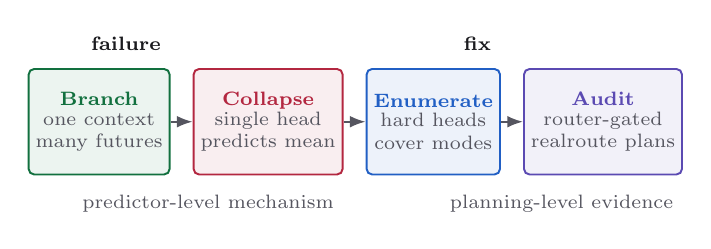
\begin{tikzpicture}[
  font=\scriptsize,
  box/.style={
    rounded corners=2pt,
    line width=0.7pt,
    minimum width=1.66cm,
    minimum height=1.34cm,
    inner sep=2.5pt,
    align=center
  },
  arr/.style={-{Latex[length=2.0mm,width=1.5mm]}, line width=0.75pt, draw=mopmuted}
]
\node[box, draw=mopgreen, fill=mopgreen!8] (a) at (0,0)
  {\textbf{\textcolor{mopgreen}{Branch}}\\[-1pt]
   \textcolor{mopmuted}{one context}\\
   \textcolor{mopmuted}{many futures}};
\node[box, draw=mopred, fill=mopred!8, right=0.28cm of a] (b)
  {\textbf{\textcolor{mopred}{Collapse}}\\[-1pt]
   \textcolor{mopmuted}{single head}\\
   \textcolor{mopmuted}{predicts mean}};
\node[box, draw=mopblue, fill=mopblue!8, right=0.28cm of b] (c)
  {\textbf{\textcolor{mopblue}{Enumerate}}\\[-1pt]
   \textcolor{mopmuted}{hard heads}\\
   \textcolor{mopmuted}{cover modes}};
\node[box, draw=moppurple, fill=moppurple!8, right=0.28cm of c] (d)
  {\textbf{\textcolor{moppurple}{Audit}}\\[-1pt]
   \textcolor{mopmuted}{router-gated}\\
   \textcolor{mopmuted}{realroute plans}};
\draw[arr] (a) -- (b);
\draw[arr] (b) -- (c);
\draw[arr] (c) -- (d);
\node[above=0.10cm of a.north east, anchor=south east, text=mopink, font=\scriptsize\bfseries]
  {failure};
\node[above=0.10cm of c.north east, anchor=south east, text=mopink, font=\scriptsize\bfseries]
  {fix};
\node[below=0.12cm of b.south east, anchor=north east, text=mopmuted, font=\scriptsize]
  {predictor-level mechanism};
\node[below=0.12cm of d.south east, anchor=north east, text=mopmuted, font=\scriptsize]
  {planning-level evidence};
\end{tikzpicture}
\caption{Argument outline. Stochastic branchings create a one-to-many latent prediction problem; a single
JEPA predictor collapses to the conditional mean, while hard-assigned predictor heads enumerate the
successor modes. The paper then audits whether those modes are actually usable for planning, rather than
merely improving multi-sample coverage.}
\label{fig:overview}
\vspace{-0.6em}
\end{figure}

\paragraph{Evidence chain.}
We prove the collapse for deterministic and gated-MoE predictors (Props.~\ref{prop:mean}
and~\ref{prop:moe}), and prove that MoP-JEPA's hard assignment is a per-context quantizer of the
successor distribution (Prop.~\ref{prop:lloyd}). We then test the mechanism before emphasizing benchmark
scores: two-step branchings produce three or four valid successor modes, the dense predictor places one
peak, and MoP-JEPA re-opens the fan-out (Fig.~\ref{fig:bimodal}); antmaze, pixel observations, ETH/UCY,
SVHN, and a DINO-WM port check that the phenomenon is not a 2-D maze artifact
(Table~\ref{tab:evidence}). Finally, we ask whether the recovered modes support planning. Single-output
planners reach only $0.02$--$0.09$ success on OGBench stitch and teleport tasks, whereas planning over our
enumerated modes recovers (Table~\ref{tab:planning}) and the recovered plans use real transitions
(Table~\ref{tab:realroute}).

\paragraph{Why the audit matters.}
Multi-prediction evaluation has a loophole: more samples can cover more outcomes without being
context-conditional enough to plan. Our protocol therefore audits everyone, ourselves first, with an
\emph{input-agnostic codebook} control, a \emph{shuffled-context} test, a \emph{router-gated} readout,
\emph{transition-precision} guards, and a \emph{verified-route} criterion in which the model proposes a
transition graph blind and ground truth is used only to check whether the route exists. This demotes raw
coverage before it adjudicates any baseline.

\paragraph{Contributions.}
(1)~\textbf{Diagnosis:} conditional-mean collapse of deterministic and gated-MoE JEPA predictors under
stochastic dynamics. (2)~\textbf{Fix:} MoP-JEPA, a hard-assignment multi-predictor head whose loss is the
classical multiple-choice / winner-take-all objective \citep{guzman2012multiple,lee2016stochastic} but
whose role here is world-model mode enumeration. (3)~\textbf{Causal evaluation:} a collapse-to-planning
measurement chain, with controls, that separates usable context-conditional modes from coverage
freeloading.

\section{Related Work}

\paragraph{JEPA world models.}
I-JEPA \citep{assran2023ijepa} and V-JEPA \citep{bardes2024vjepa} established latent-regression
prediction; DINO-WM \citep{zhou2024dinowm} and V-JEPA~2 \citep{assran2025vjepa2} use the recipe as an
action-conditioned world model for planning. Notably, the original JEPA blueprint \citep{lecun2022path}
includes a latent variable whose stated role is to carry exactly the information a multimodal future
leaves undetermined --- yet every released system above implements the predictor \emph{without} it,
deterministically. We verified this directly on the flagship: loading the released V-JEPA~2-AC checkpoint
(a $305$M-parameter action-conditioned predictor) with the authors' own code, the predictor emits a
\emph{single} next-latent per (state, action) --- the single-head design our analysis shows collapses
under stochastic dynamics. We study what that omission costs and supply the missing component in an
enumerable form; we are orthogonal to the encoder and its anti-collapse machinery \citep{bardes2022vicreg}.

\paragraph{Probabilistic JEPA.}
\citet{huang2026varjepa} argue JEPA should be probabilistic and add a variational single-Gaussian
predictive distribution; the problem framing is theirs. We benchmark their mechanism (with fixes and a
steelmanned implementation; \emph{Var-JEPA} hereafter, to avoid confusion with Meta's V-JEPA) and find
that a single Gaussian spreads but cannot separate discrete successor modes. Enumerable modes, not
samples, are what discrete search consumes.

\paragraph{MoE predictors in JEPA.}
M3-JEPA \citep{lei2024m3jepa} implements the predictor as a gated MoE fused by a weighted sum into one
output. We prove the fusion collapses identically to the single head (Prop.~\ref{prop:moe}) and confirm
this empirically; the fix is the loss (keep $K$ outputs, assign hard), not the expert count.

\paragraph{Multiple-choice and mixture regression.}
MCL/WTA \citep{guzman2012multiple,lee2016stochastic} and mixture density networks
\citep{bishop1994mixture} are classical answers to one-to-many regression. Our contribution is the JEPA
world-model instantiation, the collapse diagnosis, and the verification protocol; the
multimodal-regression literature typically reports oracle coverage without controls, which is the loophole the
protocol closes.

\paragraph{Offline GCRL (external anchor).}
OGBench's published baselines \citep{park2025ogbench,park2023hiql,wang2023qrl,eysenbach2022crl,%
ghosh2021gcbc} solve these tasks with reward-free policy learning. We do not claim to beat this line; we
report their published numbers as an external anchor at execution time and note the protocol differences.

\section{Setup and Notation}

Offline transitions $\mathcal{D}=\{(s,a,s')\}$ come from the official OGBench datasets
\citep{park2025ogbench}. An encoder $f_\theta(s)\to z\in\mathbb{R}^d$ is trained with an EMA target copy
$f_\xi$; a predictor $g$ maps $(z,a)$ to a prediction of $z'=f_\xi(s')$. Stochastic or stitched data makes
the conditional law $p(z'\mid z,a)$ multimodal: teleport cells map one $(s,a)$ to one of three fixed
destinations, and stitched datasets give one state several observed continuations (measured average
$2.1$--$2.2$ successor modes per cell). We write $c=(z,a)$ for the context; $\mu_1,\dots,\mu_M$ for the
$M$ successor-mode centers with weights $w_1,\dots,w_M$ and within-mode standard deviation $\sigma$; and
$\hat z' = z'/\lVert z'\rVert$ for normalized targets. The downstream task is goal reaching: plan to the
official evaluation goals using only the model (graph search over predicted successors, or model-predictive
control in the environment), with success judged without giving the model access to ground truth.

\section{Conditional-Mean Collapse}

\begin{prop}[deterministic predictor]\label{prop:mean}
Under squared loss the optimal single predictor is $g^*(c)=\mathbb{E}[z'\mid c]=\sum_m w_m\mu_m$; its error
is lower-bounded by the between-mode variance, and for well-separated modes
($\min_{m\neq m'}\lVert\mu_m-\mu_{m'}\rVert\gg\sigma$) the optimum lies far from every mode. Under cosine
loss with normalized targets and a unit-norm predictor, the exact minimizer is
$u^*=\mathbb{E}[\hat z']/\lVert\mathbb{E}[\hat z']\rVert$, whose similarity to every mode direction is
bounded away from $1$ whenever the mode directions are mutually separated (Lemma~1, technical appendix).
\end{prop}

\begin{prop}[gated MoE]\label{prop:moe}
A weighted sum $\hat g(c)=\sum_k \pi_k(c)\,g_k(c)$ outputs a single vector; its objective equals
Prop.~\ref{prop:mean}'s with $v=\hat g(c)$. Additional experts and router capacity change which single
vector is reachable, not how many are output.
\end{prop}

\begin{prop}[best-of-$K$]\label{prop:lloyd}
Assume $M$ well-separated modes with bounded within-mode variance, mode weights bounded away from zero,
$K\geq M$, and predictor heads with sufficient capacity. Then
$L(\{g_k\})=\mathbb{E}\!\left[\min_k\lVert g_k(c)-z'\rVert^2\right]$ is, per context, the $K$-means
distortion of $p(\cdot\mid c)$ \citep{lloyd1982least}, and every optimum assigns at least one head to each
mode, with distortion approaching the within-mode variance. A context-only router trained on the winning
index estimates the mode weights. The load-balance and router cross-entropy terms used in training are
regularizers outside this statement.
\end{prop}

Proofs and the precise separation conditions are in the technical appendix. Figure~\ref{fig:bimodal} measures Props.~\ref{prop:mean} and \ref{prop:lloyd} in the latent
space of trained models; Figure~\ref{fig:maze} shows the same models' decoded predictions on the maze
(a controlled bimodal illustration is in the technical appendix); the $K$-sweep of
Figure~\ref{fig:ksweep} measures the rise-until-$M$-then-plateau behavior that Prop.~\ref{prop:lloyd}
predicts.

\begin{figure}[t]
\centering
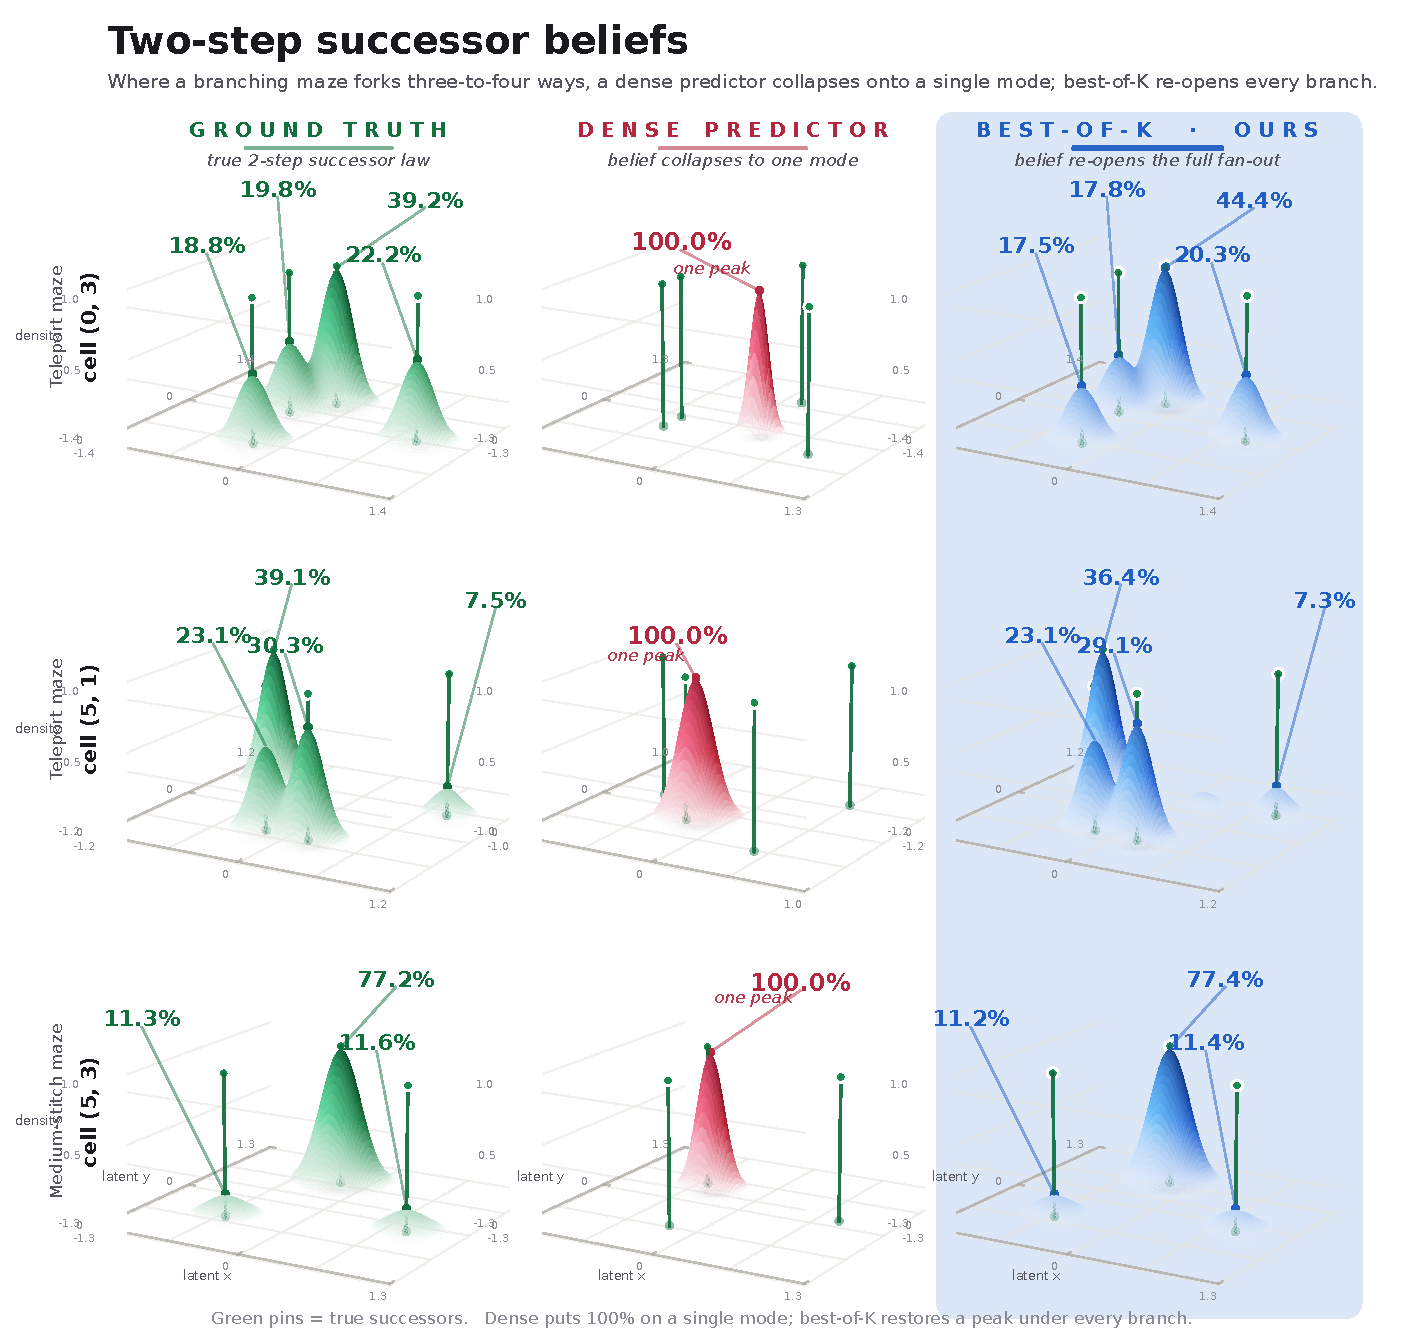
\includegraphics[width=\columnwidth]{fig_beliefs_2step_editorial.pdf}
\caption{Two-step successor beliefs at high-branching cells. \textbf{Rows:} three cells whose two-step
successor law has three or four valid modes. \textbf{Columns:} empirical ground truth (green), the dense
single predictor (red), and MoP-JEPA (blue). Each panel is the local 2-D latent plane spanned by the
true successor embeddings; floor axes give the latent coordinates, and the vertical coordinate is
unit-normalized predictive density. Green pins mark true successor latents. Percentages in the left column
are empirical two-step branch frequencies; percentages in the right column are router weights $\pi_k$ for
active heads. The dense predictor collapses to one peak, while MoP-JEPA re-opens the multimodal fan-out
with one predicted peak per branch.}
\label{fig:bimodal}
\end{figure}

\begin{figure}[t]
\centering
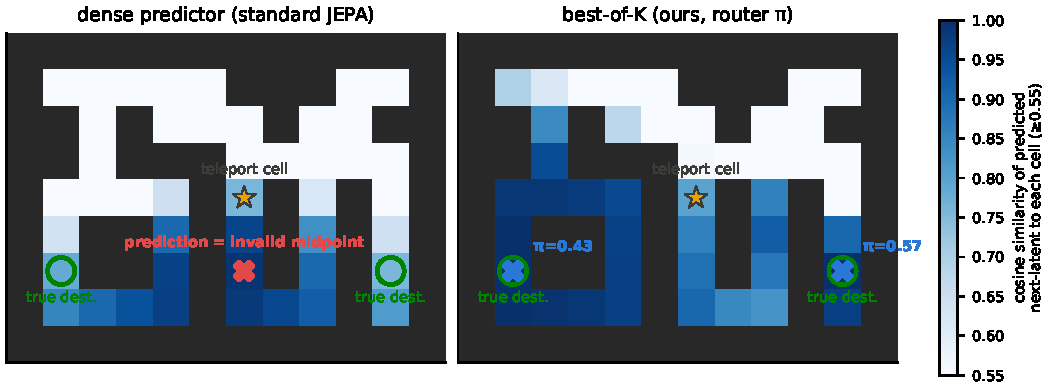
\includegraphics[width=\columnwidth]{fig_maze.pdf}
\caption{The collapse and the fix on official data (OGBench pointmaze-teleport; trained models). Heat:
cosine similarity of the predicted next-latent to each cell's latent. Left: at the teleport cell (star)
with two destinations (green circles), the dense predictor decodes to the invalid midpoint cell (red
cross). Right: our two router-activated heads (blue crosses) land on both true destinations with weights
$\pi=0.57/0.43$, close to the empirical branch frequencies $0.42/0.40$. The same geometry viewed in latent space is in the technical appendix.}
\label{fig:maze}
\end{figure}

\section{Method}

\paragraph{Variables and standard JEPA objective.}
Let $\mathcal{D}=\{(s_i,a_i,s_i^+)\}_{i=1}^N$ be an offline transition dataset, where
$s_i\in\mathcal{S}$ is the current observation or state, $a_i\in\mathcal{A}\subseteq\mathbb{R}^{p}$ is the
action, and $s_i^+$ is the observed successor. In domains without actions, $a_i$ is omitted and the context
below is just the current latent. The online encoder is $f_\theta:\mathcal{S}\to\mathbb{R}^d$ and the
target encoder is an exponential-moving-average copy $f_\xi:\mathcal{S}\to\mathbb{R}^d$. For a minibatch
$\mathcal{B}$, define
\begin{equation}
\begin{aligned}
z_i &= \frac{f_\theta(s_i)}{\lVert f_\theta(s_i)\rVert_2},\\
z_i^+ &= \operatorname{sg}\!\left(
\frac{f_\xi(s_i^+)}{\lVert f_\xi(s_i^+)\rVert_2}\right),\\
c_i &= [z_i,a_i],
\end{aligned}
\end{equation}
where $z_i\in\mathbb{R}^d$ is the online context latent, $z_i^+\in\mathbb{R}^d$ is the stop-gradient target
latent, $c_i\in\mathbb{R}^{d+p}$ is the predictor input, and $\operatorname{sg}(\cdot)$ stops gradients into
the target branch. A standard deterministic JEPA predictor is a function
$g_\phi:\mathbb{R}^{d+p}\to\mathbb{R}^d$ trained by latent regression,
\begin{equation}
\begin{aligned}
\mathcal{L}_{\mathrm{dense}}(\theta,\phi;\xi)
&= \frac{1}{|\mathcal{B}|}\sum_{i\in\mathcal{B}}
\ell\!\left(\bar g_\phi(c_i), z_i^+\right),\\
\bar g_\phi(c)&=\frac{g_\phi(c)}{\lVert g_\phi(c)\rVert_2},
\end{aligned}
\end{equation}
with cosine distance $\ell(u,v)=1-u^\top v$ in our implementation. After each optimizer step on
$(\theta,\phi)$, the target encoder is updated by
\begin{equation}
\xi \leftarrow \tau \xi + (1-\tau)\theta ,
\end{equation}
with EMA momentum $\tau$ (we use $\tau=0.996$). Thus the encoder side is the usual JEPA recipe; the only
architectural change below is the predictor.

\paragraph{Mixture-of-Predictors parameterization.}
MoP-JEPA replaces the single predictor $g_\phi$ with $K$ predictor heads
$\{g_{\phi_k}\}_{k=1}^K$, each mapping the same context $c_i$ to one candidate successor latent. It also
learns a context-only router $r_\psi:\mathbb{R}^{d+p}\to\mathbb{R}^K$. For each example $i$ and head $k$,
define
\begin{equation}
\begin{aligned}
u_{ik} &= \frac{g_{\phi_k}(c_i)}{\lVert g_{\phi_k}(c_i)\rVert_2},\\
\pi_{ik} &= \frac{\exp(r_\psi(c_i)_k)}
{\sum_{j=1}^K \exp(r_\psi(c_i)_j)},\\
d_{ik} &= \ell(u_{ik},z_i^+).
\end{aligned}
\end{equation}
Here $u_{ik}$ is the $k$th predicted successor latent, $\pi_{ik}$ is the router's deployment-time weight for
that head, and $d_{ik}$ is the distance from that head to the observed target. The router is deliberately
restricted to $c_i$; it never sees $z_i^+$ and therefore cannot choose a head by peeking at the future.

\paragraph{Hard-assignment objective.}
For fixed predictions, the latent target assigns itself to the closest head,
\begin{equation}
k_i^*=\arg\min_{1\leq k\leq K} d_{ik},\qquad
\gamma_{ik}=\mathbf{1}[k=k_i^*],
\end{equation}
where $k_i^*$ is the winning head and $\gamma_{ik}$ is its one-hot assignment. The MoP-JEPA loss is
\begin{equation}
\begin{aligned}
\mathcal{L}_{\mathrm{MoP}}
&= \frac{1}{|\mathcal{B}|}\sum_{i\in\mathcal{B}}\sum_{k=1}^K
\gamma_{ik} d_{ik}
+ \lambda_{\mathrm{route}}\,
\frac{1}{|\mathcal{B}|}\sum_{i\in\mathcal{B}} -\log \pi_{i k_i^*}\\
&\quad + \lambda_{\mathrm{bal}}\,
\sum_{k=1}^K \bar\gamma_k \log (K\bar\gamma_k),
\end{aligned}
\label{eq:mop-loss}
\end{equation}
where $\bar\gamma_k=|\mathcal{B}|^{-1}\sum_{i\in\mathcal{B}}\gamma_{ik}$ is the minibatch usage of head
$k$, $\lambda_{\mathrm{route}}$ weights the router cross-entropy, and $\lambda_{\mathrm{bal}}$ weights the
load-balancing penalty $\operatorname{KL}(\bar\gamma\Vert\mathrm{Unif}(K))$. The first term is the
best-of-$K$ JEPA regression loss. It gives gradient only to the winning head for each target, so with
assignments fixed the update for head $k$ is exactly the ordinary JEPA predictor update restricted to the
subset $\{i:k_i^*=k\}$. The second term trains the router to predict the hard assignment from the context
alone; the third prevents unused heads during minibatch optimization. When $K=1$, Eq.~\eqref{eq:mop-loss}
reduces to $\mathcal{L}_{\mathrm{dense}}$ up to constants.

This is a hard-EM procedure in latent space. The assignment step chooses the nearest current head
($k_i^*$), and the update step moves that head toward the assigned target while fitting the router to the
same assignments. Under the multimodal conditional law in Prop.~\ref{prop:lloyd}, this objective is the
empirical $K$-means distortion of $p(z^+\mid c)$; hence the heads specialize to distinct successor modes
instead of averaging them into one vector.

\paragraph{Baselines and protocol.}
We compare predictor \emph{mechanisms}, not codebases. Because none of these predictors has been applied
to JEPA world-model planning before, no prior numbers exist for this setting; we therefore reimplement each
under one common protocol --- identical encoder, offline data, EMA target, and planner --- so that the
predictor head is the only variable. The arms are: \emph{dense} ($K{=}1$, standard JEPA);
\emph{M3-JEPA} \citep{lei2024m3jepa}, its gated mixture-of-experts fused by a weighted sum; \emph{Var-JEPA}
\citep{huang2026varjepa}, a variational single-Gaussian predictor (steelmanned: cosine-trained mean,
residual-calibrated $\sigma$, $1/\sqrt d$-scaled sampling); \emph{MDN} \citep{bishop1994mixture}, a soft
mixture with load balancing (best of a $K\times\lambda$ grid); and \emph{MoP-JEPA} (ours). These are
faithful same-protocol reimplementations, not runs of the authors' released code; the published
OGBench GCRL numbers we quote later are used only as an external anchor, never as a same-protocol
comparison.

\paragraph{Prediction interface.}
At test time the model receives only $(s,a)$. It computes $z=f_\theta(s)/\lVert f_\theta(s)\rVert_2$,
$c=[z,a]$, and emits the set
\begin{equation}
\begin{aligned}
\mathcal{P}(s,a)&=\{(u_k,\pi_k)\}_{k=1}^K,\\
u_k&=\frac{g_{\phi_k}(c)}{\lVert g_{\phi_k}(c)\rVert_2},\\
\pi_k&=\operatorname{softmax}(r_\psi(c))_k .
\end{aligned}
\end{equation}
The output is therefore an enumerable successor set in one forward pass, not samples from a post-hoc
decoder and not a weighted average. A downstream planner or evaluator can consume all heads, or only router-
active heads above a fixed threshold, without access to the realized successor.

\section{Verification Protocol}

Multi-prediction can look good by covering outcomes for free, so every positive result is audited. We use
\emph{planAll} for model-internal graph searchability and \emph{official-goal success} for held-out goals,
but the load-bearing metric is \emph{realroute}: the model first proposes a transition graph blind, and
ground truth is used only afterward to check whether a route made entirely of real transitions exists
inside that proposal. \emph{Transition precision} guards against graph inflation by non-existent edges, and
\emph{execution success} runs the planner closed-loop in the environment. Three controls separate usable
mode enumeration from freeloading: an input-agnostic \emph{codebook}, an off-context \emph{shuffle} test,
and \emph{router gating}, where only heads with context-predicted mass $\pi_k>0.5/K$ count.

\section{Experiments}

\paragraph{Setup.}
Official OGBench offline datasets: pointmaze-medium-stitch, pointmaze-large-stitch,
pointmaze-teleport-navigate, and antmaze-teleport (29-D). Leak-free evaluation: coordinate features (no
cell-identity memorization) and $20\%$ of unique transitions held out of training. Five seeds for
planning, three for coverage and execution; tables give mean$\pm$std over seeds and figures show per-seed
points. No metric gives the model access to ground truth at decision time.

\subsection{Evidence Chain and Generality}

The central question is not whether one predictor variant wins one maze benchmark, but whether the same
mechanism repeats across stochastic predictors, branching degrees, and domains. Table~\ref{tab:evidence}
summarizes the evidence chain we test before reporting planner scores; Fig.~\ref{fig:evidence} plots the
three main diagnostics.

\begin{table}[t]
\centering
\scriptsize
\begin{tabular}{@{}p{0.27\columnwidth}p{0.64\columnwidth}@{}}
\toprule
Link in the chain & Evidence in the paper \\
\midrule
Collapse & Dense/gated-MoE emit one latent mean; the decoded maze state is an invalid midpoint
(Figs.~\ref{fig:bimodal}, \ref{fig:maze}). \\
Specialization & MoP-JEPA re-opens three/four-way fan-outs; independently trained heads collapse to the
same mean. \\
Branching complexity & Coverage rises until $K$ matches the mode count; two-step cells expose the
rare-mode ceiling. \\
Generality & ETH/UCY, SVHN, antmaze, pixel observations, and DINO-WM show the same mechanism beyond 2-D
point mazes. \\
Planning consequence & Realroute verifies that enumerated modes form a searchable graph of real
transitions. \\
\bottomrule
\end{tabular}
\caption{The paper's evidence chain: stochastic targets create conditional-mean collapse; hard-assigned
heads specialize to modes; mode enumeration restores a transition graph that can be audited by planning.}
\label{tab:evidence}
\end{table}

\begin{figure*}[t]
\centering
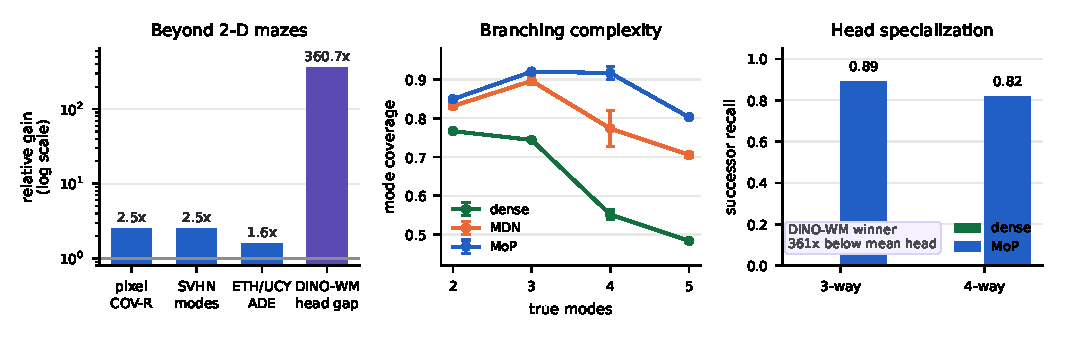
\includegraphics[width=\textwidth]{fig_evidence_chain.pdf}
\caption{\textbf{Evidence chain before benchmark scores.} Left: beyond 2-D mazes, MoP improves the
appropriate domain metric (coverage for pixel/SVHN, inverse ADE for ETH/UCY); in DINO-WM, the winning head
is hundreds of times closer than the mean head, showing specialization in the official world-model code.
Middle: as the true number of modes grows in a controlled conformer branch sweep, dense coverage degrades
fast, MDN partially covers, and hard-assigned MoP remains highest. Right: on real two-step maze branchings,
dense recovers no successor modes while MoP recovers most 3/4-way successors; this is the empirical
specialization predicted by Prop.~\ref{prop:lloyd}.}
\label{fig:evidence}
\end{figure*}

The same collapse and fix appear beyond low-dimensional mazes. On a genuine JEPA latent forecaster
(ETH/UCY pedestrians \citep{pellegrini2009eth}, leave-one-scene-out) the mixture beats the codebook control
on every scene and seed ($0.053$ vs.\ $0.070$ vs.\ dense $0.118$, shuffle $2.0\times$), and on raw
multimodal regression it improves pedestrian forecasting ($+37.7\%$) and image inpainting ($+24.1\%$),
both fully context-conditional under the controls. Conversely, standard masked-SSL pretext is
near-deterministic given context: there is no collapse to fix and multiple predictors tie the single one.
This scopes the contribution precisely: JEPA as a forecaster or world model of genuinely multimodal
futures.

The mechanism also transfers to a second codebase and to image observations. Porting the head into
\emph{DINO-WM}'s official world model \citep{zhou2024dinowm} is a one-line predictor override
(\texttt{predictor=mixture}) with no other pipeline change; it trains as a drop-in, and its heads
specialize rather than duplicate --- on held-out pixel point-maze the winning head's next-latent error is
two orders of magnitude below the head average, with $\approx\!2$ heads active per state, matching the
maze's local branching factor. On masked-digit \emph{SVHN} (real images, bottom-half inpainting), the
deterministic head realizes only $0.31$ of the conditional digit-modes while the mixture heads realize
$0.78$ ($2.5\times$, 3 seeds); density and ensemble baselines reach $0.85$--$0.89$ but expose no
enumerable, router-gated successor set to plan through.

Finally, the collapse and its fix persist as the number of futures grows. Aggregated over \emph{all}
three- and four-way \emph{two-step} maze cells ($3$ seeds, technical appendix), MoP-JEPA recovers
$82$--$88\%$ of the successors while the dense predictor recovers \emph{none}: its single mean prediction
lands between the modes, on no valid state. The hard-assigned heads retain even low-probability ($<\!10\%$)
successors; the residual gap is a rare-mode ceiling at four-way branching (a single tail mode missed in
some cells), consistent with the winner-take-all limit we report in the limitations.

\subsection{Planning on the Predicted Graph}

\begin{table}[t]
\centering
\small
\begin{tabular}{@{}lccc@{}}
\toprule
planAll $\uparrow$ & med-stitch & teleport & large-stitch \\
\midrule
dense (JEPA) & .084{\tiny$\pm$.03} & .037{\tiny$\pm$.01} & .016{\tiny$\pm$.01} \\
M3-JEPA & .075{\tiny$\pm$.02} & .036{\tiny$\pm$.01} & .031{\tiny$\pm$.01} \\
Var-JEPA & .085{\tiny$\pm$.01} & .035{\tiny$\pm$.01} & .033{\tiny$\pm$.00} \\
MDN & .566{\tiny$\pm$.20} & .512{\tiny$\pm$.12} & .717$^{\dagger}${\tiny$\pm$.12} \\
\textbf{MoP-JEPA (ours)} & \textbf{.851}{\tiny$\pm$.08} & \textbf{.748}{\tiny$\pm$.09} & .386{\tiny$\pm$.45} \\
\midrule
codebook (control) & .267{\tiny$\pm$.02} & .167{\tiny$\pm$.02} & .149{\tiny$\pm$.04} \\
\bottomrule
\end{tabular}
\caption{planAll (searchability of the predicted graph; 5 seeds). Official-goal success shows the same
ordering (Fig.~\ref{fig:planning}); the codebook control reaches near-zero official-goal success
($0.00$--$0.15$) despite its nonzero planAll. $^{\dagger}$MDN's large-stitch score depends on
low-precision predicted edges and is adjudicated in Table~\ref{tab:realroute}.}
\label{tab:planning}
\end{table}

\begin{figure}[t]
\centering
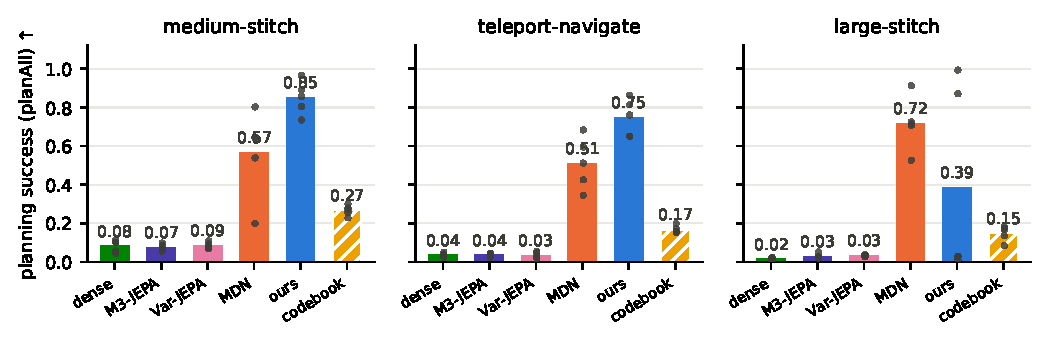
\includegraphics[width=\columnwidth]{fig_planning.pdf}
\caption{planAll by arm (bars: mean; dots: seeds). The codebook control (hatched) shows that coverage
alone does not plan: it maxes raw coverage (Table~\ref{tab:coverage}) yet reaches near-zero official-goal
success.}
\label{fig:planning}
\end{figure}

Table~\ref{tab:planning}: deterministic, gated-MoE, and Var-JEPA predictors reach $0.02$--$0.09$,
consistent with Props.~\ref{prop:mean}--\ref{prop:moe}; ours reaches up to $0.85$.

\subsection{Adjudication: Verified Routes}

MDN's raw numbers depend on predicted edges that do not exist: its transition precision is
$0.14$--$0.21$ (ours $0.42$--$0.56$), and graph search will happily route through hallucinated walls.
Under \emph{realroute}, all three mazes favor ours (Table~\ref{tab:realroute},
Fig.~\ref{fig:realroute}). The paired advantage over MDN is statistically significant on medium-stitch
(bootstrap $95\%$ CI of the per-seed difference $[0.06, 0.18]$) and teleport ($[0.07, 0.24]$); on
large-stitch the mean favors ours but the CI includes zero at five seeds, reflecting the seed-bimodality
we report below. Under fully matched capacity and training ($K{=}16$, $60$k steps, $5$ seeds, both arms' best
load-balance settings) the large-stitch verdict is unambiguous: ours reaches realroute $0.208$ vs.\ MDN's
$0.095$ ($2.2\times$), with MDN's found rate high ($0.88$) but precision low ($0.21$) --- it routes through
non-existent edges --- against our $0.42$ precision. More capacity buys the MDN more hallucinated edges,
not more real routes.

\begin{table}[t]
\centering
\small
\begin{tabular}{@{}lccc@{}}
\toprule
realroute $\uparrow$ & dense & MDN & \textbf{MoP-JEPA} \\
\midrule
medium-stitch & .083{\tiny$\pm$.03} & .134{\tiny$\pm$.03} & \textbf{.247}{\tiny$\pm$.08} \\
teleport-navigate & .035{\tiny$\pm$.01} & .039{\tiny$\pm$.01} & \textbf{.192}{\tiny$\pm$.09} \\
large-stitch & .016{\tiny$\pm$.01} & .057{\tiny$\pm$.03} & \textbf{.139}{\tiny$\pm$.15} \\
\bottomrule
\end{tabular}
\caption{Verified planning: a real route must exist inside the model's blind proposal (5 seeds). The
failure modes separate: dense is precise but mode-collapsed (a graph too sparse to route); MDN covers but
its routes rely on non-existent edges; MoP-JEPA is the only predictor whose proposed graph contains
real routes at a useful rate.}
\label{tab:realroute}
\end{table}

\begin{figure}[t]
\centering
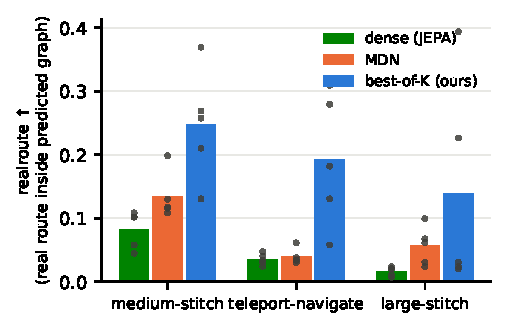
\includegraphics[width=0.9\columnwidth]{fig_realroute.pdf}
\caption{Verified routes by task (bars: mean; dots: seeds).}
\label{fig:realroute}
\end{figure}

\begin{figure}[t]
\centering
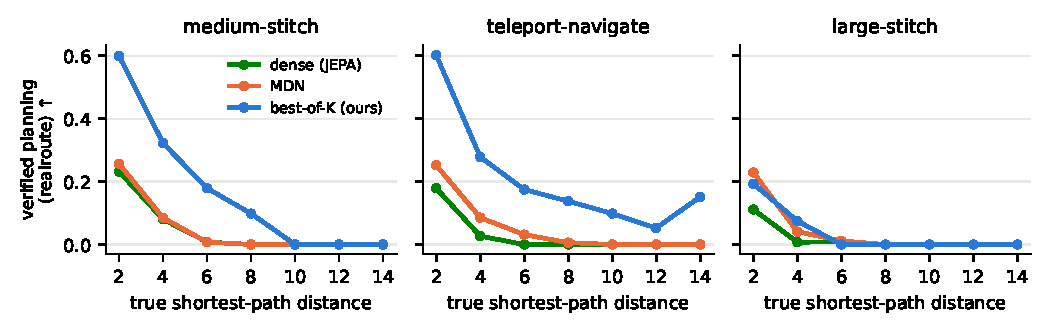
\includegraphics[width=\columnwidth]{fig_horizon.pdf}
\caption{Verified (realroute) success vs.\ the true shortest-path distance of the goal (3 seeds). The
multimodal advantage compounds with horizon: on teleport, ours still plans at distances $10$--$14$ where
both baselines reach zero by $d{=}6$; on large-stitch all arms decay quickly.}
\label{fig:horizon}
\end{figure}

\paragraph{Long horizons.}
Fig.~\ref{fig:horizon}: at distance $6$ on medium-stitch ours retains $0.18$ verified success versus
MDN's $0.01$; on teleport, where long routes cross the stochastic branching repeatedly, ours holds
$0.05$--$0.15$ out to distance $14$ while both baselines reach zero by distance $6$--$8$. Mode errors
compound multiplicatively with rollout depth, which is why a mode-faithful one-step predictor is the
load-bearing requirement for long-horizon planning.

\paragraph{Is the MDN under-tuned?}
A fairness grid over components $K\in\{8,16\}$ and load-balance weight $\lambda\in\{0,0.01,0.1\}$
(learned $\sigma$ throughout, 3 seeds each) leaves the ordering unchanged on every task: the strongest
variant reaches realroute $0.125$ on medium (ours $0.247$) and $0.114$ on teleport (ours $0.192$). On
large-stitch, strong load-balancing genuinely helps MDN (best variant $0.191$); under fully matched
capacity and training it remains behind ours.

\subsection{Verified Planning Across the JEPA Predictor Family}

\begin{table*}[t]
\centering
\small
\begin{tabular}{@{}lccc|cc@{}}
\toprule
& \multicolumn{3}{c}{\textbf{verified planning (realroute)} $\uparrow$}
& \multicolumn{2}{c}{execution $\uparrow$} \\
\cmidrule(lr){2-4}\cmidrule(lr){5-6}
JEPA predictor (same encoder, data, planner) & med-stitch & teleport & large-stitch & med & large \\
\midrule
dense (standard JEPA) & .083 & .035 & .016 & .27 & .13 \\
M3-JEPA & .075 & .036 & .031 & --- & --- \\
Var-JEPA (variational) & .034 & .001 & .033 & --- & --- \\
MDN (best of a $K\times\lambda$ grid) & .134 & .039 & .095 & .87 & .27 \\
\textbf{MoP-JEPA (ours)} & \textbf{.247} & \textbf{.192} & \textbf{.208} & .67 & \textbf{.33} \\
\bottomrule
\end{tabular}
\caption{\textbf{Within the JEPA world-model family --- same encoder, data, and planner, only the
predictor changes --- ours wins verified planning on all three mazes ($2$--$5\times$; 5 seeds.)}
Left block (realroute): a plan counts only if the model's blindly-proposed transition graph contains a
route of \emph{real} transitions, so coverage cannot be freeloaded. Dense/gated-MoE/Var-JEPA are
mode-collapsed (Props.~\ref{prop:mean}--\ref{prop:moe}); MDN covers but routes through non-existent edges
(precision $0.14$--$0.21$ vs.\ ours $0.42$--$0.56$; large-stitch adjudicated at matched $K{=}16$/$60$k
steps). Right block: real-environment execution success (official \texttt{info['success']}, our
replanning executor); MDN's higher medium-stitch number is the executor's online repair compensating its
low-precision graph, which is precisely why model fidelity is judged by realroute.
\emph{External context:} on large-stitch our execution ($33$) sits second among the seven published
OGBench offline-GCRL baselines \citep{park2025ogbench} (QRL $84$; then ours, GCIQL $31$, HIQL $13$,
GCIVL $12$, GCBC $7$, CRL $0$) --- notable for a generic world model plus search rather than a
policy trained end-to-end for the benchmark.}
\label{tab:exec}
\end{table*}

The family comparison is same-protocol by construction: every arm shares the encoder, the offline data,
and the planner, and differs only in the predictor head, so Table~\ref{tab:exec} isolates the effect of
the predictor's output distribution. Our executor is verified sound ($15/15$ on true paths; on a truth
graph corrupted with $10\%$ false edges, replanning lifts success $0.40\to1.00$), and a uniform-edge-cost
ablation leaves all execution rankings unchanged. The published-baseline numbers are quoted only as
external context, not a same-protocol comparison; the load-bearing result is that a one-line predictor
change turns a world model that cannot plan into one that plans verifiably.

\subsection{Coverage of Stochastic Dynamics}

\begin{table}[t]
\centering
\small
\begin{tabular}{@{}lcccc@{}}
\toprule
pointmaze-teleport & raw & $\pi$-gated & COV-P & shuffle \\
\midrule
dense & .244{\tiny$\pm$.03} & .244{\tiny$\pm$.03} & .733 & 2.4$\times$ \\
M3-JEPA & .242{\tiny$\pm$.04} & .242{\tiny$\pm$.04} & .727 & 1.4$\times$ \\
Var-JEPA & .001{\tiny$\pm$.00} & .001{\tiny$\pm$.00} & .000 & --- \\
MDN & .596{\tiny$\pm$.02} & .292{\tiny$\pm$.01} & .864 & 1.8$\times$ \\
\textbf{MoP-JEPA} & .997{\tiny$\pm$.00} & \textbf{.632}{\tiny$\pm$.22} & \textbf{.924} & \textbf{2.4$\times$} \\
\midrule
codebook & 1.00{\tiny$\pm$.00} & 1.00$^{\ddagger}$ & .417 & 1.0$\times$ \\
\bottomrule
\end{tabular}
\caption{Coverage of the three teleport destinations (COV-R, 3 seeds). $^{\ddagger}$The codebook has no
context and cannot be gated. Raw coverage can be freeloaded (the codebook maxes it), so raw COV-R is a
diagnostic, never a headline; under the router-gated readout ours is the only arm simultaneously high on
coverage, precision, and context-conditionality.}
\label{tab:coverage}
\end{table}

\begin{figure}[t]
\centering
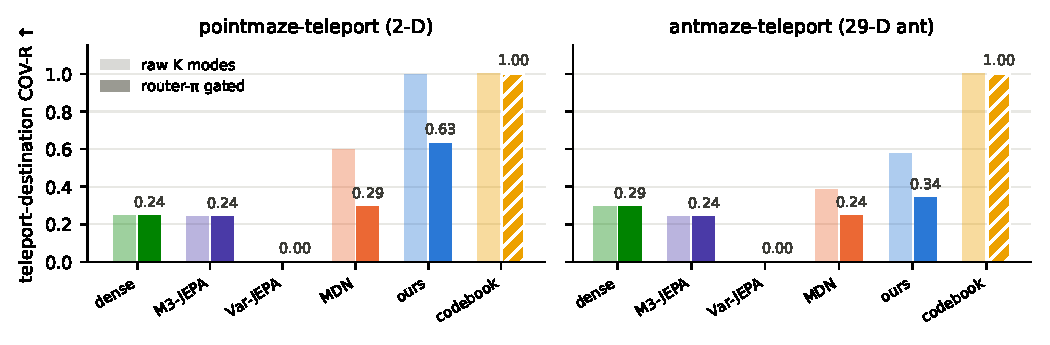
\includegraphics[width=\columnwidth]{fig_coverage.pdf}
\caption{Raw (light) vs.\ router-gated (solid) coverage on pointmaze and 29-D antmaze.}
\label{fig:coverage}
\end{figure}

Destinations are fixed global states, so the input-agnostic codebook maxes raw COV-R at $1.0$; our own
protocol flags naive coverage as freeloading. The verdict is threshold-insensitive: sweeping the gate over
$t\in[1/64,1/4]$, our gated coverage degrades gracefully ($0.74\to0.40$) while precision
($\approx0.92$) and shuffle leakage ($\approx0.26$) stay flat, and every baseline is invariant or pinned
below. On \textbf{antmaze-teleport} (29-D ant, destinations as manifolds of 32 real samples) the ranking
persists with honest attenuation: ours $0.576$ raw, about $2\times$ dense ($0.294$) and $1.5\times$ MDN
($0.386$); gated $0.342$ at $0.86$ precision; Var-JEPA $0$. On \textbf{pixel observations}
(visual-antmaze-teleport, $64{\times}64{\times}3$; CNN JEPA trained from scratch, teleport transitions
oversampled identically for every arm), the ranking again persists: ours $0.613$ raw COV-R vs.\
$0.24$--$0.27$ for every baseline ($2.4\times$), with partial mode recovery (gated $\approx 1$ of 3
modes at $0.97$ precision). High-dimensional and pixel-level JEPA world models capture the branching
direction but not yet full mode-fidelity; closing that gap is open.

\subsection{Summary and Ablations}

\begin{table}[t]
\centering
\small
\begin{tabular}{@{}lccccc@{}}
\toprule
 & modes & COV-R & prec. & real- & exec \\
 & enum.? & (gated) & & route & (hard) \\
\midrule
dense & no & .24 & high & 0/3 & .13 \\
M3-JEPA & no & .24 & high & 0/3 & --- \\
Var-JEPA & samples & .00 & --- & 0/3 & --- \\
MDN & soft & .29 & .14--.21 & 0/3 & .27 \\
\textbf{MoP-JEPA} & \textbf{yes} & \textbf{.63} & .42--.56 & \textbf{3/3} & \textbf{.33} \\
codebook & static & n/a & --- & 0/3 & --- \\
\bottomrule
\end{tabular}
\caption{Trade-off summary. Each baseline misses a different requirement of a plannable stochastic world
model; MoP-JEPA is the only arm that enumerates context-conditional modes with usable precision and
leads verified planning on all three mazes.}
\label{tab:scoreboard}
\end{table}

\begin{figure}[t]
\centering
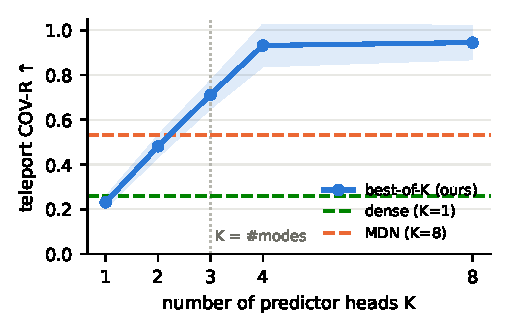
\includegraphics[width=0.85\columnwidth]{fig_ksweep.pdf}
\caption{$K$-sweep on real data (teleport COV-R): coverage rises until $K$ equals the number of modes,
then plateaus, with no penalty for over-provisioning, as Prop.~\ref{prop:lloyd} predicts.}
\label{fig:ksweep}
\end{figure}

\paragraph{$K$-sweep (real data).} Teleport COV-R rises from $0.231$ at $K{=}1$ (matching dense $0.258$)
to $0.712$ at $K{=}3$ (the number of modes) and plateaus at $0.945$ by $K{=}8$ (MDN at $K{=}8$: $0.531$).

\paragraph{Design ablations.} An explicit head-separation loss is redundant (WTA already separates, and it
can hurt recall). Slow soft-to-hard annealing over $80\%$ of training drags every head toward the mean; a
fast warmup accelerates small-model convergence dramatically while plain hard EM is already sufficient at
full scale. \textbf{An ensemble of $K$ independently trained heads (no assignment) collapses entirely}:
realroute $0.03$--$0.10$, at dense level, with zero spread across heads --- each head converges to the same
conditional mean, Prop.~\ref{prop:mean} applied $K$ times. Independence is not diversity; hard assignment
is the load-bearing design choice.

\subsection{The Protocol Fires Where It Should}

\emph{It audits the strongest baseline}: MDN's raw planning scores are traced to non-existent predicted
edges (\S Adjudication). \emph{It audits us}: raw coverage is demoted as freeloadable
(Table~\ref{tab:coverage}). \emph{It detects metric artifacts}: on antmaze, full-observation destination
centroids score every arm and every control at exactly zero, the fingerprint of an off-manifold reference
point (ant joints are arbitrary at a fixed-$xy$ destination), which we caught and replaced with
real-sample manifolds. \emph{It rejects illusory multimodality}: on road-constrained taxi forecasting an
apparent $+36\%$ gain is $84\%$ reproducible by the codebook (shuffle $1.23\times$) and is rejected; on
persistence-dominated next-frame video no gain is claimed. The verdict tracks whether futures genuinely
branch, which is what makes the positive results trustworthy.

\section{Discussion and Limitations}

\paragraph{Why this matters for scaling JEPA world models.}
Video- and robot-scale world models \citep{assran2025vjepa2,zhou2024dinowm} are trained on data where
stochasticity is the rule. Our results indicate that the deterministic predictor's failure there is not
graceful: the error concentrates on exactly the branchings a planner must resolve, and it silently
produces states that do not exist. The broader lesson is that a stochastic world model should expose a
set-valued transition interface, not only a latent expectation. MoP-JEPA is one minimal implementation of
that interface: a head-level change, orthogonal to encoder architecture and scale, that yields enumerable
branch outcomes with calibrated router weights. The verification protocol is architecture-agnostic: any
world model that emits multiple futures (mixture, variational, diffusion, or generative) can be audited
with the same suite, and we would encourage its adoption wherever multi-sample prediction numbers are reported.

\paragraph{Limitations.}
The claim concerns the transition distribution and what it enables; single-shot selection of an aleatoric
branch is impossible for any model and is not claimed. WTA optimization on the hardest maze is
seed-bimodal, and at four-way two-step branching a rare ($<\!10\%$) successor can fall
below head activation and be missed (full four-mode recovery in $37\%$ of such cells); annealing does not
fix it at scale, an explicit head-repulsion
regularizer hurts, and head-wise learning rates or replay biased toward rare modes remain untested. Mazes are low-dimensional
state spaces; the 29-D ant extends the mechanism with attenuation, and the DINO-WM port
confirms the head-level fix on pixel observations, though scaling the verification protocol to video- and
robot-scale world models remains future work. Comparisons within the predictor family are same-protocol reimplementations (no prior numbers
exist for these predictors in this setting); the published-baseline anchor is quoted, not rerun, and is
not a same-protocol comparison.

\section{Conclusion}

A deterministic JEPA world model cannot represent a stochastic branching: it predicts a latent expectation
where planning needs enumerable futures. We prove this conditional-mean collapse, show it across branch
counts and beyond 2-D mazes, and measure the planning failure it causes. Hard-assigned predictors recover
one successor mode each, turning the predictor output from a single invalid average into a searchable
transition set; verified planning succeeds when that set contains real routes. The method is deliberately
minimal, but the point is broader: stochastic JEPA world models need mode enumeration, and claims about
multimodal prediction should be audited for context-conditional, real-transition structure rather than raw
oracle coverage.

% AAAI wraps \bibliography in \FloatBarrier; the local draft \FloatBarrier is a
% \clearpage, which leaves a large blank gap after the conclusion. Keep the
% references attached to the conclusion instead.
\begingroup
\let\FloatBarrier\relax
\bibliography{refs}
\endgroup

\end{document}
